%%!TEX root = main.tex
\section{Learning to predict outdoor lighting}
\label{sec:cnn}

\subsection{Dataset organization}

To train the CNN, we first apply the optimization procedure from sec.~\ref{sec:optimization} to 38,814 high resolution outdoor panoramas in the SUN360~\cite{xiao-cvpr-12} database. We then extract 7 photos from each panorama using a standard pinhole camera model and randomly sampling its parameters: its elevation with respect to the horizon in $[-20^\circ, 20^\circ]$, azimuth in $[-180^\circ, 180^\circ]$, and vertical field of view in $[35^\circ, 68^\circ]$. The resulting photos are bilinearly interpolated from the panorama to a resolution $320 \times 240$, and used directly to train the CNN described in the next section. This results in a dataset of 271,698 pairs of photos and their corresponding lighting parameters, which is split into (261,288 / 1,751 / 8,659) subsets for (train / validation / test). These splits were computed on the panoramas to ensure that photos taken from the same panorama do not end up in training and test. Example panoramas and corresponding photos are shown in fig.~\ref{fig:evaluation_example_sun_position}. 

\subsection{Architecture}

We adopt a standard feed-forward convolutional neural network to learn the relationship between the input image $I$ and the lighting parameters. As shown in fig.~\ref{fig:cnn-architecture}, its architecture is composed of 7 convolutional layers, followed by a fully-connected layer. It then splits into two separate heads: one for estimating the sun position (left in fig.~\ref{fig:cnn-architecture}), and one for the sky and camera parameters (right in fig.~\ref{fig:cnn-architecture}). 

The sun position head outputs a probability distribution over the likely sun positions $\mathbf{s}$ by discretizing the sky hemisphere into 160 bins (5 for elevation, 32 for azimuth), and outputs a value for each of these bins. This was also done in~\cite{lalonde-ijcv-12}. As opposed to regressing the sun position directly, this has the advantage of indicating other regions believed to be likely sun positions in the prediction, as illustrated in fig.~\ref{fig:evaluation_example_sun_position} below. The parameters head directly regresses a 4-vector of parameters $\mathbf{q}$: 2 for the sky ($\omega$, $t$), and 2 for the camera (elevation and field of view). The ELU activation function~\cite{clevert-iclr-16} and batch normalization~\cite{ioffe-jmlr-15} are used at the output of every layer. 

\subsection{Training details}

We define the loss to be optimized as the sum of two losses, one for each head: 
%
\begin{equation}
\mathcal{L}(\mathbf{s}^*, \mathbf{q}^*, \mathbf{s}, \mathbf{q}) = \mathcal{L}(\mathbf{s}^*, \mathbf{s}) + \beta \mathcal{L}(\mathbf{q}^*, \mathbf{q}) \,,
\label{eqn:ch3_loss}
\end{equation}
%
where $\beta = 160$ to compensate for the number of bins in $\mathbf{s}$. We experimentally validated that this value provides gradients with similar magnitude between both neural network heads. The target sun position $\mathbf{s}^*$ is computed for each bin $\mathbf{s}_j$ as 
%
\begin{equation}
\mathbf{s}^*_j = \exp(\kappa \mathbf{l}_s^{*\mathsf{T}} \mathbf{l}_j) \,,
\label{eqn:vmf}
\end{equation}
%
and normalized so that $\sum_j \mathbf{s}^*_j = 1$. The equation in (\ref{eqn:vmf}) represents a von Mises-Fisher distribution~\cite{banerjee-jmlr-05} centered about the ground truth sun position $\mathbf{l}_s$. Since the network must predict a confident value around the sun position, we set $\kappa = 80$. The target parameters $\mathbf{q}^*$ are simply the ground truth sky and camera parameters. 

% Note to yan: netPT9 epoch 5
\begin{figure}[t]
    \centering
    \footnotesize
    \setlength{\tabcolsep}{1pt}
    \begin{tabular}{cc}
    \multicolumn{2}{c}{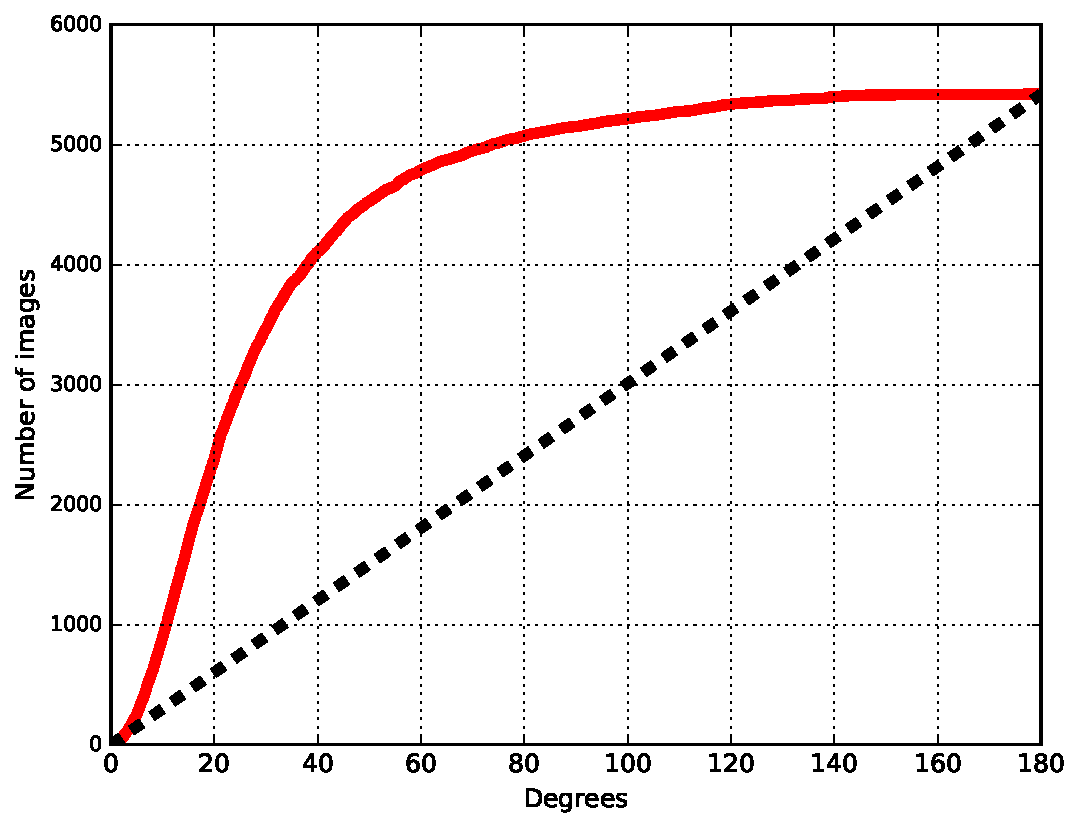
\includegraphics[width=0.5\linewidth]{./figures/evaluation_performances/cdf_sunpos_both.pdf}} \\
    \multicolumn{2}{c}{(a) Angular error} \\
    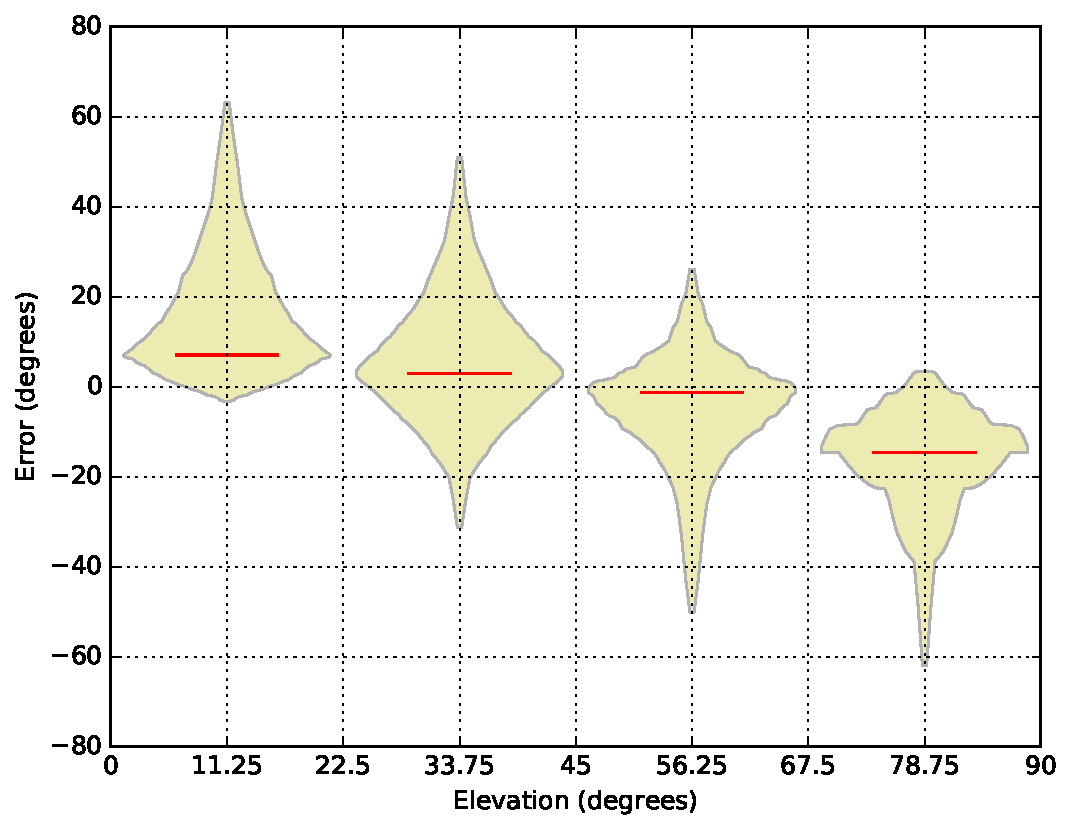
\includegraphics[width=0.48\linewidth]{./figures/evaluation_performances/box-percentile_plot_el.pdf} & 
    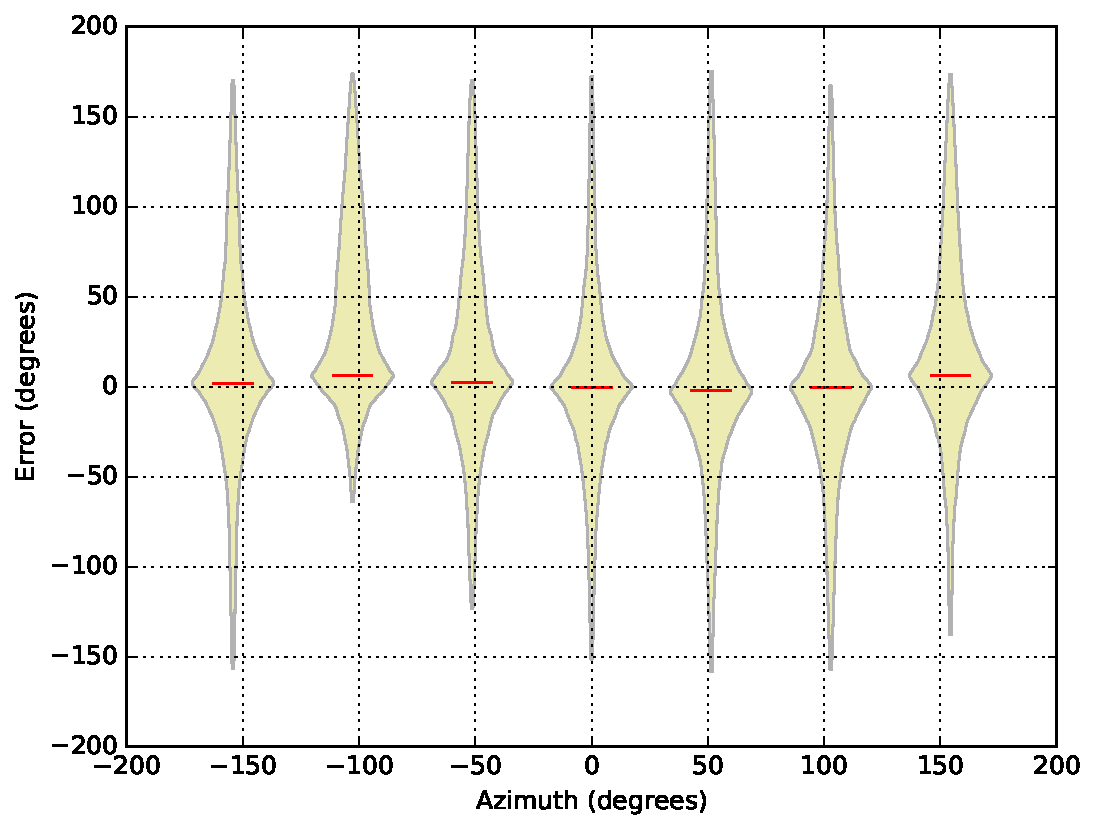
\includegraphics[width=0.48\linewidth]{./figures/evaluation_performances/box-percentile_plot_az.pdf} \\
    (b) Elevation error & (c) Azimuthal error
    \end{tabular}
    \vspace{.5em}
    \caption[Quantitative evaluation of sun position estimation]{Quantitative evaluation of sun position estimation on all 8659 images in the SUN360 test set. (a) The cumulative distribution function of the angular error on the sun position. The estimation error as function of the sun elevation (b) and (c) azimuth relative to the camera (0\degree ~means the sun is in front of the camera). The last two figures are displayed as ``box-percentile plots''~\cite{esty-jss-03}, where the envelope of each bin represents the percentile and the median is shown as a red bar.% The performance decrease at high sun elevation may be attributable to a lack of such occurrences in the training dataset.
    }
    \label{fig:evaluation_performance_sun_position}
\end{figure} 

\begin{figure}[!th]
    \centering
    \footnotesize
    \setlength{\tabcolsep}{1pt}
    \begin{tabular}{cc}
    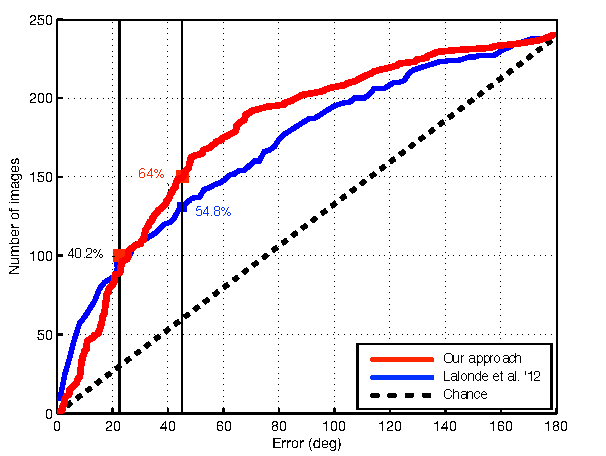
\includegraphics[height=5cm]{figures/compare_jf12/lalonde-db-margin.pdf} & 
    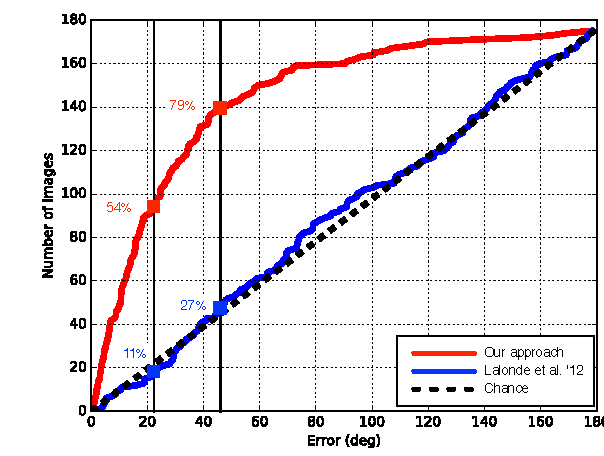
\includegraphics[height=5cm]{figures/compare_jf12/sun360-db-margin.pdf} \\
    (a) Dataset from~\cite{lalonde-ijcv-12} &
    (b) Subset of SUN360 test set
    \end{tabular}
    \vspace{.5em} 
    \caption[Performance comparison on an urban dataset]{Comparison with the method of Lalonde et al.~\cite{lalonde-ijcv-12} showing the cumulative sun azimuth estimation error on (a) their original dataset of urban scenes, and (b) a 176-image subset from the SUN360 test set. (a) While our method has similar error in an octant (less than $22.5^\circ)$, the precision in a quadrant (less than $45^\circ$) significantly improves by approximately 10\%. However, this dataset contains only urban scenes which carry many of the explicit cues sought by~\cite{lalonde-ijcv-12}. (b) The 176-images SUN360 test subset contains much more challenging images where methods based on the detection of explicit urban cues (as in~\cite{lalonde-ijcv-12}) fail. Our deep learning based approach remains robust and achieves high performance on both datasets.}
    \label{fig:comparison-lalonde12}
\end{figure}

We use a MSE loss for $\mathcal{L}(\mathbf{q}^*, \mathbf{q})$, and a Kullback-Leibler (KL) divergence loss for the sun position $\mathcal{L}(\mathbf{s}^*, \mathbf{s})$. Using the KL divergence is needed because we wish the network to learn a \emph{distribution} over the sun positions, rather than the most likely position. 

The loss in (\ref{eqn:ch3_loss}) is minimized via stochastic gradient descent using the Adam optimizer~\cite{kingma-iclr-15} with an initial learning rate of $\eta=0.01$. Training is done on mini-batches of 128 exemplars, and regularized via early stopping. The process typically converges in around 7--8 epochs, because our CNN is not as deep as most modern feed-forward CNN used in vision. Moreover, the high initial learning rate used combined with our large dataset further helps in reducing the number of epochs required for training.



